\documentclass[10pt,a4paper]{scrartcl}
\usepackage[utf8x]{inputenc}
\usepackage{ucs}
\usepackage{amsmath}
\usepackage{amsfonts}
\usepackage{amssymb}
\usepackage{graphicx}

\setlength{\parindent}{0mm}
\areaset{15cm}{26cm}

\newcommand{\likert}[1]{
\emph{#1}
\begin{center}
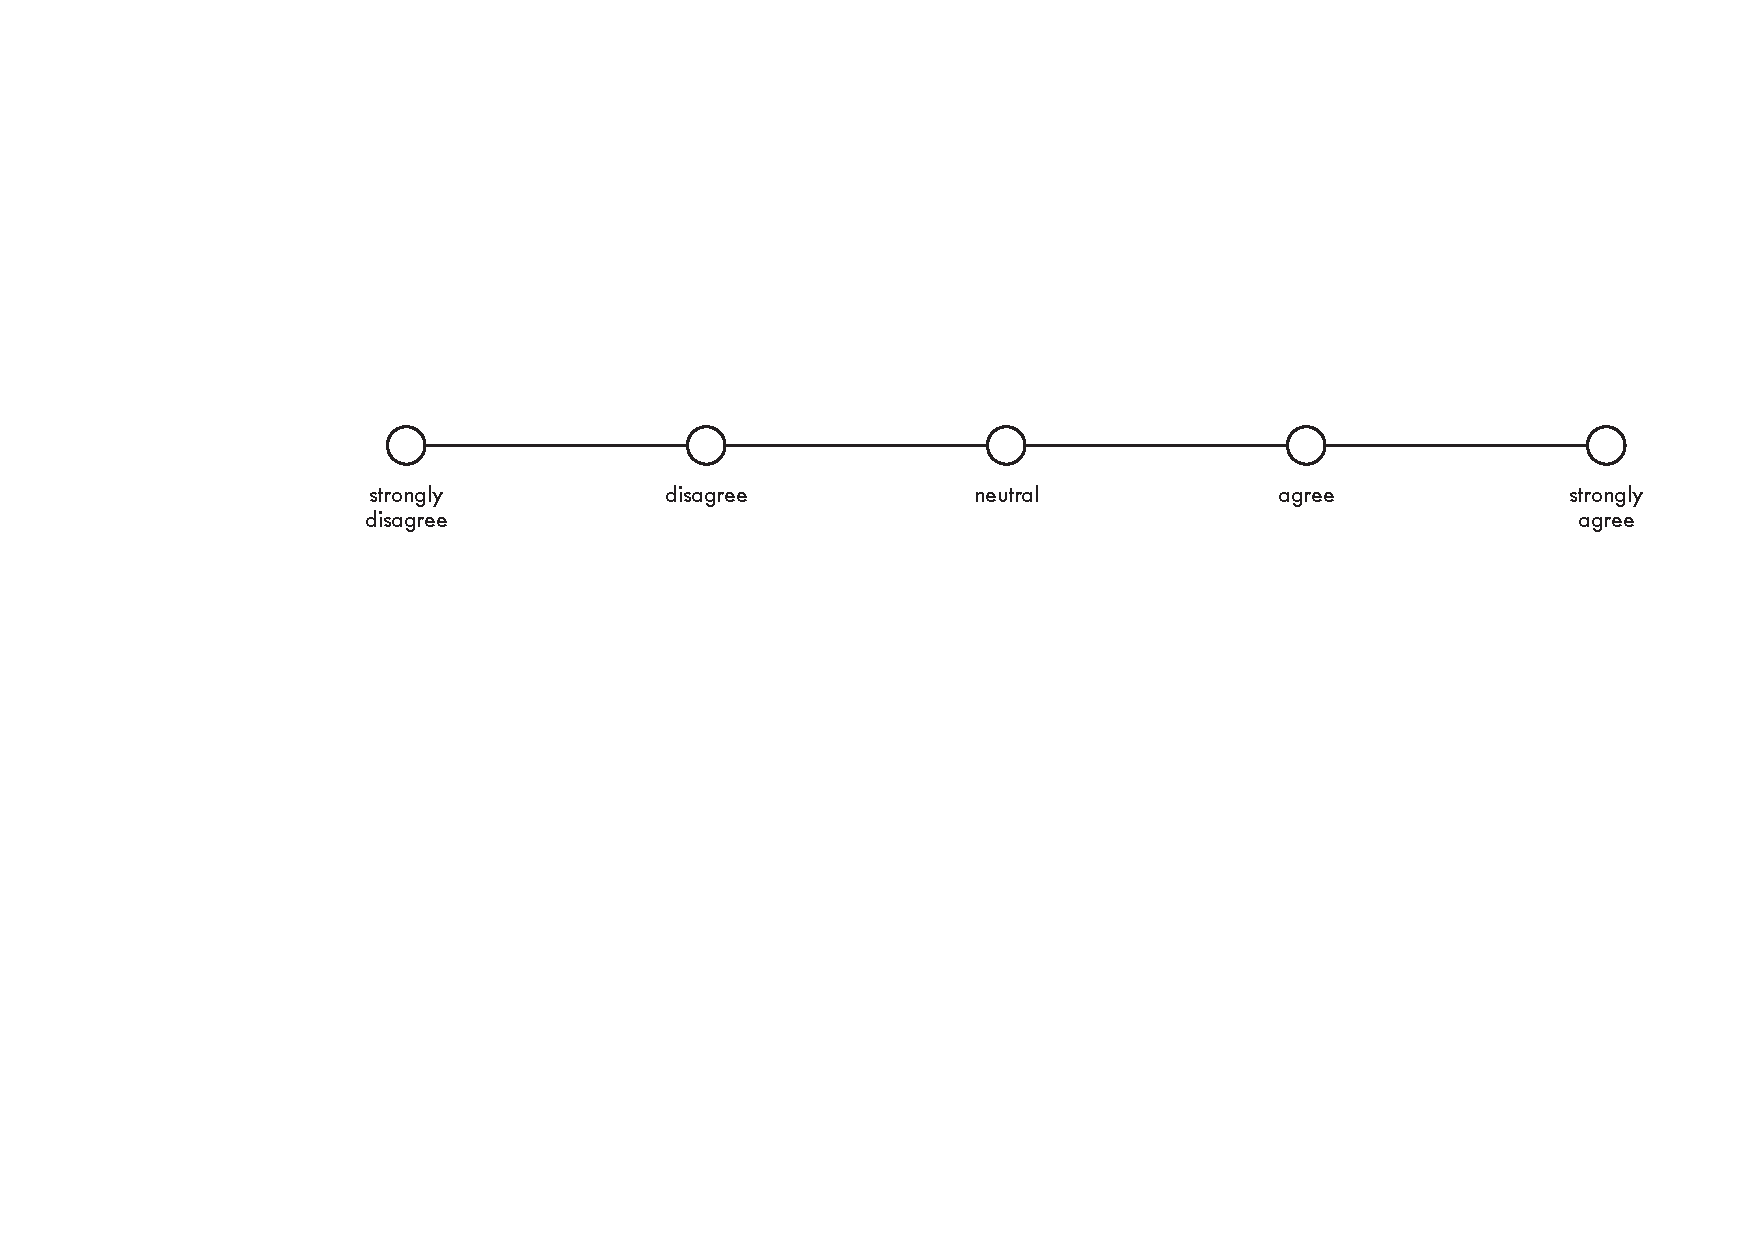
\includegraphics[width = 0.8\textwidth]{likert-5}
\end{center}
}

% #1: question text
% #2: left adjective
% #3: right adjective
\newcommand{\quis}[3]{
\emph{#1}
\quisshort{#2}{#3}
}

% #2: left adjective
% #3: right adjective
\newcommand{\quisshort}[2]{
\begin{center}
\begin{tabular}{c c c c c c c c c c c}
\multicolumn{5}{l}{\textsf{#1}} & \multicolumn{5}{r}{\textsf{#2}}\\
0 & 1 & 2 & 3 & 4 & 5 & 6 & 7 & 8 & 9\\
\end{tabular}
\end{center}
}

\title{Sputnik User Study Evaluation Form}
\author{Simon Wallner}
\date{December 12, 2011}


\begin{document}
\maketitle

% makes not much sense on a b/w printout...
% \begin{center}
% 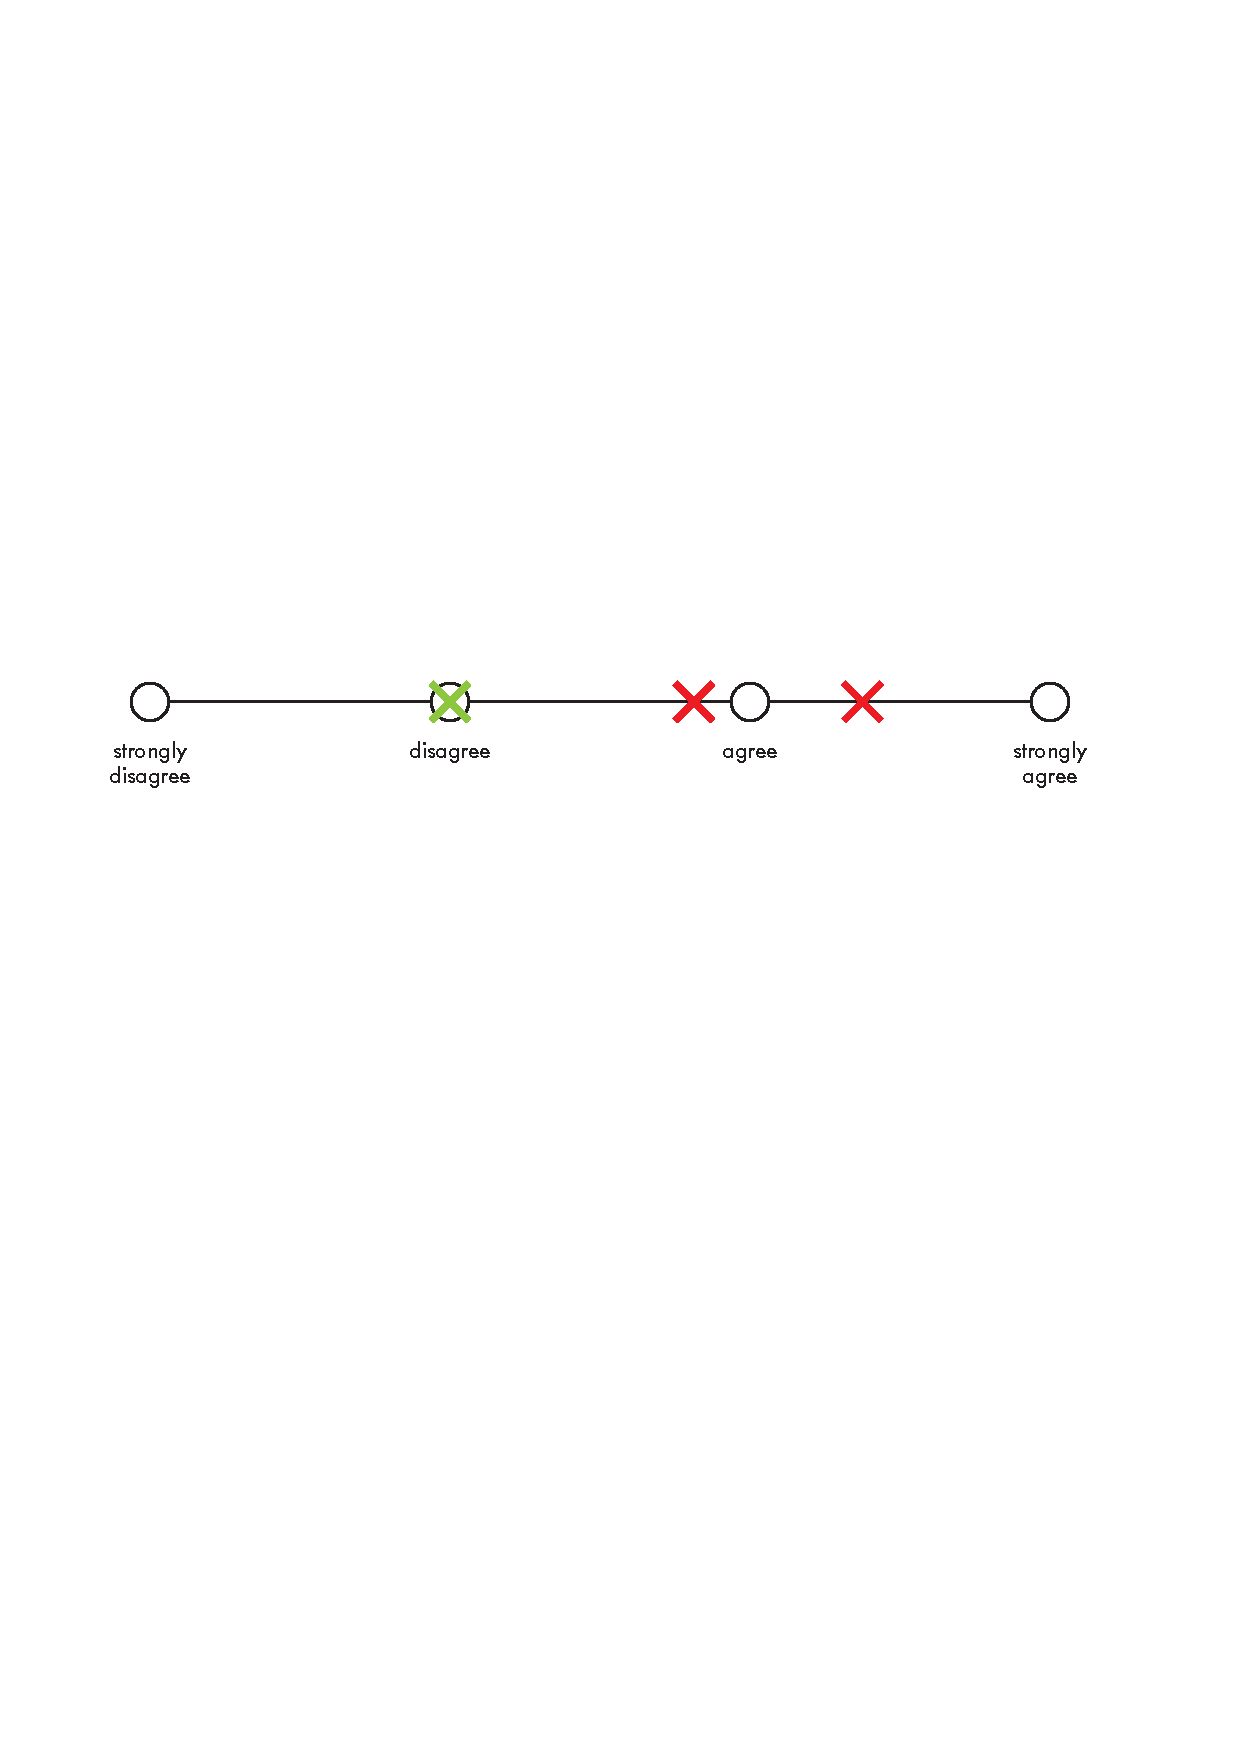
\includegraphics[width = 0.8\textwidth]{likert-4-explaination}
% \end{center}


\section{Statements}
For the following statements, please indicate your level of agreement.
\medskip

\likert{Sputnik is easy to use.}

\likert{The interface felt natural.}

\likert{I could feel the weight and physical properties of the objects.}

\likert{Using Sputnik could improve live performances.}


% \clearpage
\section{Adjectives}
For the following adjectives, please specify how they apply to Sputnik.
\medskip


\quis{Overall, Sputnik is...}{terrible}{wonderfull}
\quisshort{frustrating}{satisfying}
\quisshort{dull}{stimulating}
\quisshort{rigid}{flexible}
\quisshort{laggy}{responsive}
\quisshort{random}{controllable}
\quisshort{boring}{fun}
\end{document}